\chapter{Coulomb potential analysis in protein-GAG systems}
\label{chapter:bspred}


% I or we?
% http://english.stackexchange.com/a/24683
% http://www.researchgate.net/post/Should_I_use_either_we_or_I_in_my_thesis

In this chapter I present a simple and yet efficient method for predicting where
on a protein a GAG would most likely bind, suggesting which amino acid residues
are likely to be involved in the interaction. The method is based on numerical
simulation of the electrostatic (i.e.\ Coulomb) potential of the protein in
water solution, and manual evaluation of the topology of the Coulomb potential
in space. Subsequently, I report the findings of this method applied to IL-10.

\section{Motivation}
\label{bspred:motivation}

Classical molecular docking approaches are used for creating binding predictions
for a given receptor-ligand system. Primarily, the correctness of a prediction
depends on the quality of the underlying physical or phenomenological model, and
whether the system under investigation is within the scope of validity of the
model. Since most molecular docking methods are trained for analyzing a limited
Cartesian volume in a \textit{local} search, application to larger search spaces
such as in \textit{global} docking dramatically lowers the confidence in the
resulting prediction. Therefore, common molecular docking methods should be
applied locally, and hence require \textit{a priori} knowledge about where on
the receptor the ligand most likely binds. The decision where to center the
local search on should be based on reliable data, otherwise the docking study
might be pointless. In the best case, knowledge about the binding region (the
region on the receptor that the ligand binds to) comes from experimental data,
e.g.\ from mutagenesis or NMR studies. However, in many cases no such
experimental data is available, as is unfortunately true for the IL-10-GAG
system. In such situations, \textit{in silico} methods can be applied for
prediction of the binding region.

There is only a little amount of work published on the topic of the prediction
of protein-GAG binding regions. The proposed approaches lack a well-founded
physical model, and so far none of the approaches gained general acceptance. In
a previous work \cite{gandhi_bmp_heparin_binding_sites_2012}, PatchDock
\cite{patchdock_2002} was used for globally docking rigid heparin
oligosaccharides to different proteins. The authors carefully conclude that
\enquote{while there has been no validation of the accuracy of the PatchDock
scoring function for heparin interactions, these docking results suggest the
presence of two GAG binding sites [in one of the proteins]}. In another study
\cite{rogers_gag_prot_prot_2011}, the authors used a mixture of two docking
softwares for rigid-body docking of GAG structures \enquote{to the entire
molecular surface of the protein to locate the most favorable binding sites} and
claimed general success without further quantification or description. In
\cite{bitomsky_gag_docking_1999}, the authors report that commonly used
\enquote{docking programs (GRID, AutoDock, Dock) were able to correctly localize
the heparin binding sites on our test case proteins}. In
\cite{hp_binding_sites_mulloy_2006}, Forster and Mulloy used AutoDock version
2.4 \cite{autodock24} for globally docking rigid heparin molecules to the
proteins antithrombin and FGF2, and found that their resulting binding region
prediction agreed quite well with the regions determined experimentally. The
authors state that the method may be used as \enquote{hypothesis generation
tool} rather than for providing \enquote{details of interactions between
specific atoms}.

The above-cited studies do not provide a complete picture, but obviously some of
the established docking methods seem to be able to reflect certain properties of
protein-GAG systems. This is remarkable since none of these docking methods has
been specifically developed for GAG ligands, let alone for global docking, and
strictly spoken, when applied to protein-GAG systems, these docking methods are
applied outside their scope of validity. An issue with named studies is that
none of them provides an explanation for why a certain docking method should
yield success in protein-GAG binding region prediction. Hence, these studies
lack the capability of further enlightening the theoretical basis of protein-GAG
interaction, since a good non-arbitrary explanation would be a step towards
induction and further predictions \cite{swirski2007literature}. In scientific
theory, it is established that prediction and explanation are formally the same,
the only difference being that prediction is before the fact and explanation is
after the fact \cite{suppe1977structure}. Without proper justification (i.e.\
explanation), a prediction is not suitable for generating scientific knowledge
--- no matter if the prediction becomes corroborated or contradicted by an
empirical observation \cite{schafersman_scientific_method}.

I \textit{postulate} that the main reason for the success of docking methods in
named studies is that protein-GAG complexes are strongly driven by Coulomb
interaction, and that mentioned docking methods incorporate Coulomb interaction
with a significant weight in their scoring functions. In fact, heparin has the
highest negative charge density among biological macromolecules
\cite{capila_linhardt_hep_prot_2002}. Reviews on protein-GAG systems
\cite{essentials_glycobiology_protgags_2009,gandhi_structure_2008} stress
the role of charge-charge interaction in protein-GAG systems in general. Many
publications focusing on individual protein-GAG systems identify charge
complementary as one of the driving mechanisms of the interaction between GAG
and protein
\cite{gandhi_bmp_heparin_binding_sites_2012,faham_heparin_1996,%
pichert_characterization_2012,rogers_gag_prot_prot_2011}.

It can be concluded that the importance of Coulomb interaction is a distinctive
feature of protein-GAG systems. Notably, compared to other molecular interaction
types, the Coulomb interaction is a long range interaction and therefore
dominates all other types of interaction for larger distances. As of these
considerations, I \textit{hypothesize} that protein-GAG binding region
prediction is possible purely based on the strength and topology (i.e.\ the
shape/distribution) of the electrostatic potential in the volume surrounding the
protein. Taking this step back compared to the application of complex docking
methods is in favor of gaining scientific knowledge about the fundamental
concepts of protein-GAG interaction.

In order to determine whether the electrostatic properties alone can assist in
predicting a receptor-GAG binding region, the relation between the strength and
topology of the Coulomb potential and the actual experimentally determined GAG
binding site was investigated for a set of reference systems. From the
scientific theory point of view, the result of this study in any case further
enlightens the role of Coulomb interaction in protein-GAG systems.


\section{Method}

\subsection{Coulomb potential simulation}

The electrostatic potential of a given protein was calculated with a
finite-difference numerical solver applied to the linearized Poisson-Boltzmann
(PB) equation. The PB equation is widely used for implementing a class of
implicit solvent models to describe solvent-mediated electrostatic interactions.
These models have been demonstrated to be reliable in reproducing the energetics
when compared with explicit solvent molecular dynamics simulations and
experimental measurements for a wide range of systems \cite{honig_estatic_1995}.
In the PB model applied here, the solute (protein) is described by an
atomic-detail representation, while the solvent molecules are treated as a
continuum. The solute is modeled as a dielectric body whose shape is defined by
atomic coordinates and atomic radii. A set of point charges at the atomic
centers produces an electrostatic field in the solute region as well in the
solvent region. The overall electrostatic field is the sum of the Coulombic
field of the solute and the corresponding reaction field of the polarizable
solvent.

For calculating the overall electrostatic potential of any given protein, the
PBSA program shipped with AmberTools 13 \cite{case_amber_12} was used with
default parameters and a finite element grid spacing of \SI{1}{\angstrom}. The
atomic radii and point charges of the protein were parameterized according to
the FF99SB force field \cite{case_amber_12}. Source code modification of the
PBSA software was required for \textit{i)} writing the discretized scalar data
in compliance with the OpenDX data format \cite{opendx} and \textit{ii)} in
units of \si{\kilo\calory\per\mole\per\elementarycharge}. After patching PBSA
(and contributing those patches back to the AmberTools project), the data could
be visualized and analyzed in VMD \cite{vmd_1996}.


\subsection{Coulomb potential evaluation}

Many authors discussing the properties of a certain GAG receptor protein depict
the electrostatic potential of the protein mapped onto its molecular surface
\cite{rogers_gag_prot_prot_2011,%
mancera_mmpbsa_gags_2009,sapay_hs_growthfactors_2011,%
gandhi_bmp_heparin_binding_sites_2012,sost_heparin_2009,%
catK_cs4_crystal_structure_2008,hydrolase_gags_2011,gandhi_structure_2008,%
imberty_gag_prot_carbres_2007,gags_as_polyelectrolytes_2010}. Most of these
studies lack clear conclusions from this kind of analysis, which in my opinion
is the result of two conceptual flaws of the approach. First of all, by only
looking at the molecular surface, the properties of the potential in the volume
surrounding the protein are ignored, i.e.\ analysis of the potential which a GAG
feels when it is in the neighborhood of a protein is missed. Especially, one
misses to see how a GAG may be guided by a certain topology of the potential in
space. Secondly, an unfortunately often overseen disadvantage of the
surface-mapping approach is that the PB approximation of the electrostatic
potential is \text{most} error-prone near the dielectric boundary, i.e.\ right
on the molecular surface: Warshel et al.\ write that \enquote{the problem is not
the well-known bulk contribution from the surroundings [\dots], but the
polarization at the microscopic boundaries of the simulation spheres}
\cite{estatic_proteins_warshel_2006}.

\nomenclature{PB}{Poisson Boltzmann}

The data obtained from PBSA are the values of the electrostatic potential on the
grid centers of a three-dimensional grid, spanning a volume of a certain size
including the protein as well as its surroundings. In contrast to what is
usually done, I decided to analyze the properties of the electrostatic potential
within the entire protein-surrounding volume, \textit{i)} for working around the
uncertainty of the data near the boundary, and \textit{ii)} for not ignoring the
protein neighborhood.

Therefore, the topology and strength of the potential was analyzed with an
isosurface representation while varying the isovalue. This procedure, which will
become more clear in \cref{bspred:appl_discussion} below, allows for
understanding the shape of the potential in space as well as how strong it would
affect a ligand. Additionally, a characteristic isovalue was determined
individually for each protein under investigation, for the case where only a
small part of the isosurface is protruding into space further than the molecular
surface of the receptor. This characteristic isovalue provides an idea about the
strength of the electrostatic interaction between ligand and receptor in the
bound state. The isosurface visualization was performed using VMD
\cite{vmd_1996}.


\section{Application to reference systems}
\label{bspred:application}

The electrostatic potential of the following experimentally characterized
protein-GAG systems was analyzed: basic fibroblast growth factor (FGF2) in
complex with a heparin (HP) tetrasaccharide, PDB ID 1BFB,
\SI{1.9}{\angstrom} resolution; the CD44 hyaluronic acid binding domain in
complex with a hyaluronan (HA) heptasaccharide, PDB ID 2JCQ,
\SI{1.3}{\angstrom}; and stromal cell-derived factor-1 (SDF-1) in complex with a
HP disaccharide, PDB ID 2NWG, \SI{2.1}{\angstrom}.

% TODO: include this? Compared to effort, I dont see the value.
%Furthermore, we have applied the electrostatic potential analysis to Sclerostin
%(SOST), whose interaction with heparin has recently been investigated via NMR
%\cite{sost_heparin_2009}.


\subsection{Results and discussion}
\label{bspred:appl_discussion}

\subsubsection{FGF2}

\begin{figure}
\centering
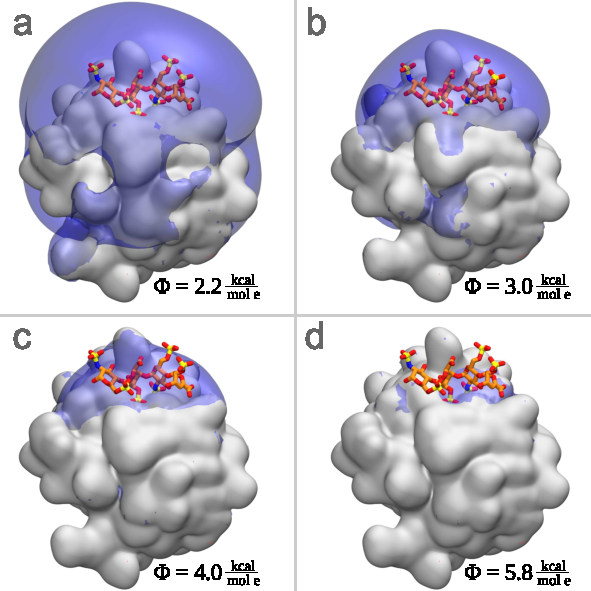
\includegraphics[width=0.9\textwidth]{gfx/bspred/fgf2_coulomb_isosurfaces_different_values_03_ds.pdf}
\caption[]{
Isosurface representation of FGF2's Coulomb potential (blue), shown for four
different isovalues $\Phi$ in increasing order. The molecular surface of FGF2
is shown in gray, the heparin ligand pose as determined experimentally is shown
as sticks with carbon atoms in orange (structure taken from PDB ID 1BFB).}
\label{fig:bspred:fgf2_multi_iso}
\end{figure}

\Cref{fig:bspred:fgf2_multi_iso} depicts the process of visualizing the
electrostatic potential of FGF2 with an isosurface representation and varying
isovalue. The four isovalues shown are positive ones, and the isosurfaces
therefore represent \textit{attraction} for GAGs. Isosurfaces for isovalues of
comparable absolute value and opposite sign are \enquote{within} the molecular
surface, i.e.\ electrostatic GAG \textit{repulsion} is negligible in case of
FGF2.

\Cref{fig:bspred:fgf2_multi_iso}a shows the isosurface corresponding to the
smallest of the four isovalues with
\SI{2.2}{\kilo\calory\per\mole\per\elementarycharge}. This is still a strong
potential, yielding significant potential energies for charged ligand molecules:
\SI{2.2}{\kilo\calory\per\mole} is almost four times larger than the thermal
energy at \SI{300}{\kelvin}. \Cref{fig:bspred:fgf2_multi_iso}a shows that FGF2
is highly polar on its global scale: in the depicted top direction, the
isosurface protrudes into space far beyond the molecular surface, whereas it
does not surpass the molecular surface at the bottom. Hence, FGF2 may interact
with GAGs over large distances (several times larger than what can be considered
a molecular contact), and with a clear preference towards one side of the
protein (the top side in the orientation as shown in
\cref{fig:bspred:fgf2_multi_iso}). Furthermore, the experimentally determined
natural heparin ligand pose is located on that side of FGF2.

Panels a, b, and c of \cref{fig:bspred:fgf2_multi_iso} visualize the process of
increasing the isovalue while observing the response of the isosurface. This
process serves two purposes. Firstly, the shape change of the isosurface with
increasing isovalue provides insight about the gradient of the potential, i.e.
the direction into which a negatively charged molecule would be \textit{guided}
by the Coulomb potential. Secondly, it allows for further narrowing down those
regions in space near the molecular surface of FGF2 where electrostatic
attraction is strongest, because the isosurface protrudes less and less into
space with increasing isovalue. Regarding directionality, the isosurface clearly
contracts itself towards a certain region on FGF2's surface, considering panels
a, b, and c of \cref{fig:bspred:fgf2_multi_iso}. It is that region where also
the experimentally determined ligand pose is to be found. Panel c shows a small
region in the neighborhood of FGF2 where the Coulomb potential is as large as
\SI{4.0}{\kilo\calory\per\mole\per\elementarycharge}, which is about seven times
stronger than the thermal energy at room temperature, considering a single test
charge. With an electrostatic attraction as strong as this and clearly no other
regions near the molecular surface of FGF2 with a comparably strong Coulomb
potential, it is unlikely that a negatively charged ligand molecule tends to
interact anywhere else with FGF2 than in that region.

\Cref{fig:bspred:fgf2_multi_iso}d shows the isosurface for what I call the
\textit{characteristic} isovalue, which (roughly) is that isovalue for which
only a residual part of the isosurface is protruding into space further than the
molecular surface of the receptor protein. The goal of this representation is to
scan the direct vicinity of the molecular surface of the protein for the regions
of strongest electrostatic attraction, and to be able to quantify that
attraction. In case of FGF2, that value was found to be about
\SI{6}{\kilo\calory\per\mole\per\elementarycharge}, which is about 10 times
larger than the thermal energy. While the isosurface representation in panel c
localizes the region of interest within a volume still larger than the size of
the heparin ligand, the isosurface in panel d narrows it further down to a more
localized volume, which might be called \enquote{hot spot}. Further inspection
shows that the position of this spot matches the position of those two sulfate
groups of the heparin ligand that are the main anchors of the interaction
between FGF2 and heparin \cite{faham_heparin_1996}. Overall, the topology of
FGF2's electrostatic potential \textit{unambiguously} suggests
\textit{one} site for potential GAG interaction, and that site very well matches
the experimentally determined one.


\subsubsection{SDF-1}

\begin{figure}
\centering
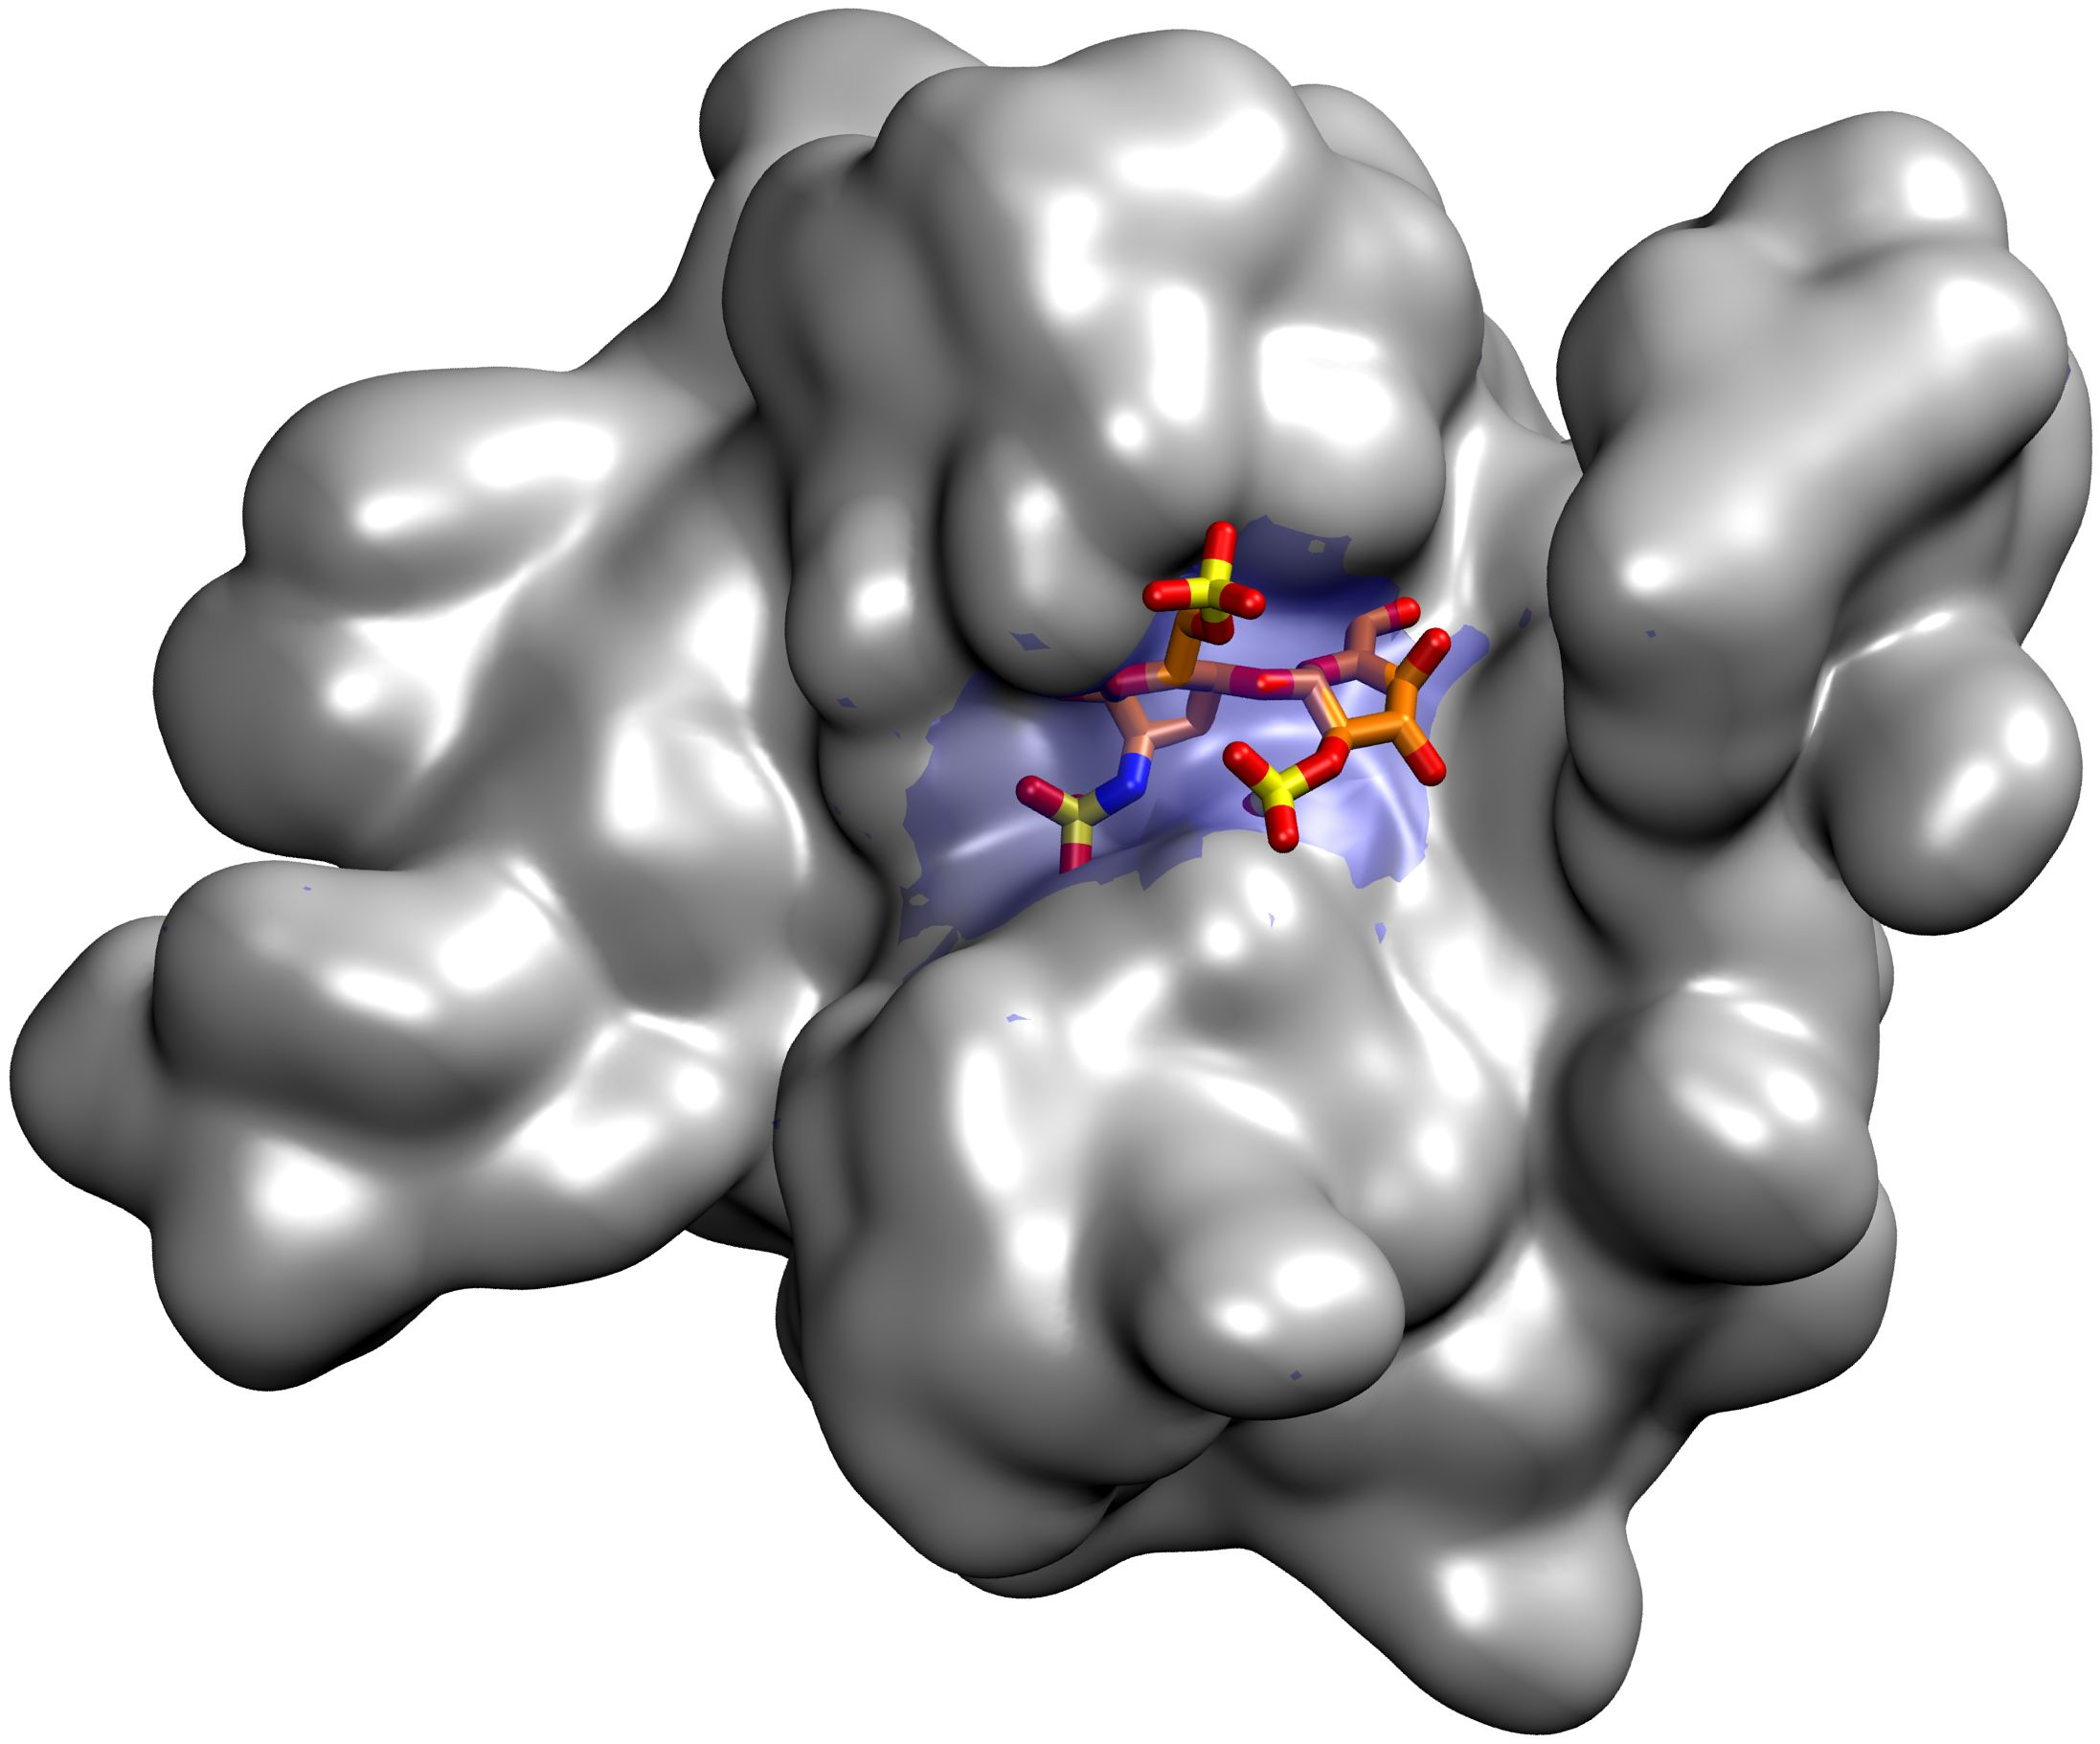
\includegraphics[width=0.7\textwidth]{gfx/bspred/sdf1_isopot_8_5_view1_rotated_jcc_pub_001.jpg}
\caption[]{
Isosurface representation of SDF-1's Coulomb potential with the characteristic
isovalue of $\Phi=\SI{8.5}{\kilo\calory\per\mole\per\elementarycharge}$ (blue).
The molecular surface of the SDF-1 dimer is shown in gray, the heparin ligand as
determined experimentally is shown in stick representation with carbon atoms in
orange (structure taken from PDB ID 2NWG).}
\label{fig:bspred:sdf1_estatic}
\end{figure}

\Cref{fig:bspred:sdf1_estatic} shows the isosurface of SDF-1's Coulomb potential
corresponding to its characteristic isovalue
$\Phi=\SI{8.5}{\kilo\calory\per\mole\per\elementarycharge}$. It can be seen that
the measured ligand pose matches the region of strongest electrostatic
attraction. Another important observation is that the characteristic isovalue is
significantly larger than in case of FGF2, meaning that the electrostatic
attraction of SDF-1 in the indicated region is stronger. In fact, SDF-1 displays
the largest characteristic isovalue I have come across during the analysis of
various different protein-GAG systems. The spatial arrangement of positively
charged residues in the shape of a cleft produces an environment in which the
attractive potential from the two sides of the cleft adds up in the center,
yielding a stronger electrostatic potential than possible with a one-sided
interaction only.

Variation of the isovalue and observing the corresponding response of the
isosurface, although not depicted here, has provided very similar conclusions as
in case of FGF2: all indicators point towards \textit{one} region on SDF-1 with
a very strong electrostatic attraction at its core, as well as the ability to
attract a GAG molecule over long distances. As in case of FGF2, the topology of
SDF-1's electrostatic potential unambiguously suggests one site for potential
GAG interaction, and that site matches the experimentally confirmed one.


\subsubsection{CD44 hyaluronic acid binding domain}

\begin{figure}
\centering
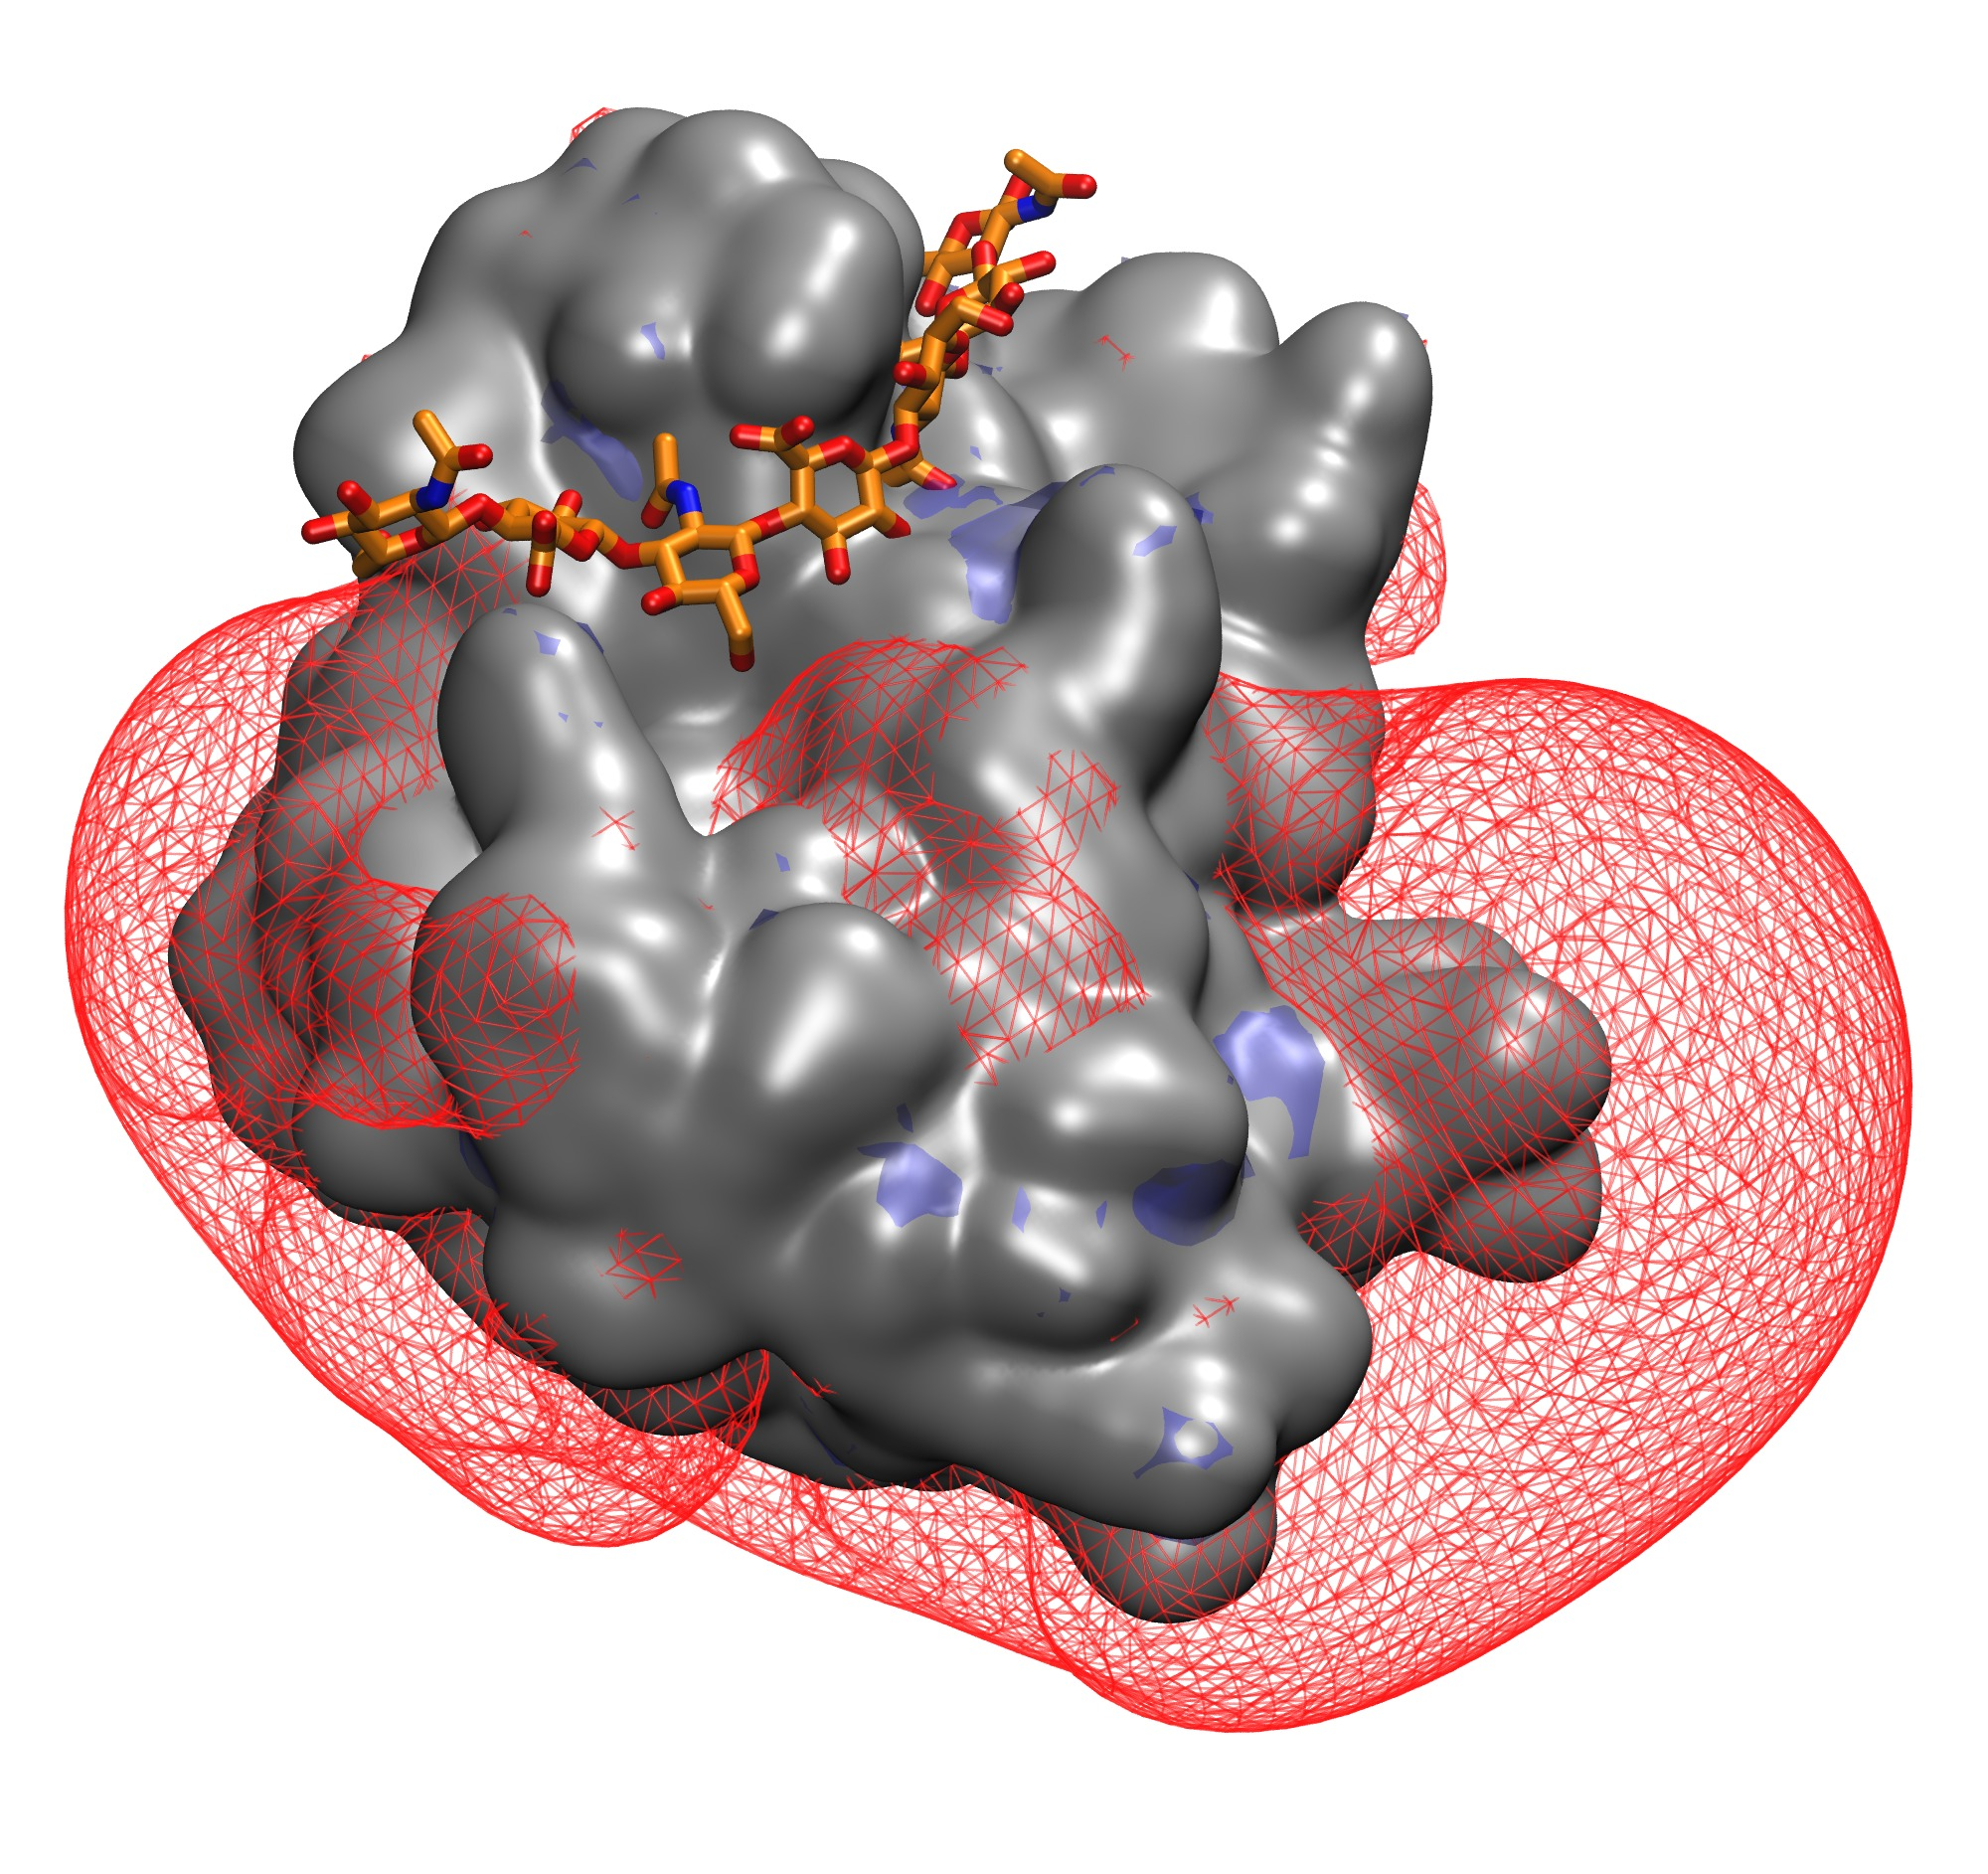
\includegraphics[width=0.7\textwidth]{gfx/bspred/2JCQ_isopot500_ligand_view1.jpg}
\caption[]{
Isosurface representation of CD44's Coulomb potential with the isovalues
$\Phi=\pm\SI{1.5}{\kilo\calory\per\mole\per\elementarycharge}$ (blue: attractive
for negative charges, red: repulsive for negative charges). The molecular
surface of the hyaluronic acid binding domain of CD44 is shown in gray, the
hyaluronan heptasaccharide ligand in the pose as determined experimentally is
shown in stick representation with carbon atoms in orange (structure taken from
PDB ID 2JCQ).}
\label{fig:bspred:cd44_estatic}
\end{figure}

CD44's interaction with hyaluronan is fundamentally different from the SDF-1-HP
and FGF2-HP systems. \Cref{fig:bspred:cd44_estatic} shows that even for the
quite small isovalue of \SI{1.5}{\kilo\calory\per\mole\per\elementarycharge}
(compared to the previously discussed systems), there is almost no (blue)
isosurface visible, meaning that the protein has no long-range electrostatic
attraction for GAGs. In direct vicinity to CD44's molecular surface some small
patches representing weak attraction for negative charges are observable.
However, their location is rather scattered. The main observation for the
CD44-HA system is that most parts of the protein have a slightly repulsive
Coulomb potential. Considering how far certain parts of the isosurface for
\SI{-1.5}{\kilo\calory\per\mole\per\elementarycharge} protrude into space, it
can be concluded that the net repulsion takes effect over longer distances.
While there seems to be a (weak) net repulsion for GAGs, there also is a larger
region on the protein surface which appears to be neutral from the electrostatic
point of view, with neither of both isosurfaces piercing through the molecular
surface of CD44. It is that region where hyaluronan was experimentally shown to
bind to CD44 (see
\cref{fig:bspred:cd44_estatic}).

For the CD44-HA system, the main conclusion is that analysis of the
electrostatic potential fits the binding pose obtained experimentally in the
sense that there is \textit{no contradiction}. When taking a close look, the
experimentally obtained binding site contains most of the scattered patches
representing attraction for negative charges mentioned above. Furthermore, it
makes sense that the hyaluronan does not bind in one of those regions that have
been identified as being explicitly repulsive for negative charges. However,
purely based on the electrostatic potential data one would \textit{not} have
been able to pinpoint a certain region as being particularly likely to attract
GAGs. The major reason for being unable to narrow down a region is that a
\textit{distinct} region of \textit{significant} electrostatic attraction is
missing. Accordingly, the authors of \cite{cd44_hya_2007} point out that CD44-HA
system is \enquote{dominated by hydrogen bonds and van der Waals forces rather
than electrostatic interactions}, a quite special characteristic among
protein-GAG systems.


\subsubsection{Reliability of the method, and its
eligibility for generating scientific knowledge}

When describing the concepts of protein-GAG interaction in all generality,
Coulomb interaction is one of the major determinants. Therefore, I claim that
evaluation of the Coulomb potential of a protein receptor alone is a systematic
and simple approach for predicting where on a protein a GAG would bind ---
\textit{if} it binds. This is an important distinction from predicting whether a
protein binds GAGs or not, which Coulomb potential analysis alone can surely not
do reliably.

The most important aspect to discuss when predicting the behavior of a system is
the \textit{certainty} of the prediction. The huge advantage of the method
presented here seems to be that it \textit{intrinsically} provides a good
estimate about the certainty of its own prediction, i.e.\ this method is
unlikely to generate false-positives. For example, the data about CD44 shown
above does not allow for stating anything more definite than \enquote{we can not
tell where a GAG would bind, however it will most likely not bind in the
repulsive regions}. At the same time the data regarding FGF2 and SDF-2 provide
undeniable support that GAGs bind where the Coulomb potential points towards,
especially regarding the large characteristic electrostatic potential isovalues
in proximity of the molecular surface. The main conclusion is that if a
\textit{distinct} region of \textit{significant} electrostatic attraction can be
observed, then this is the place where a GAG would most likely bind. If the
electrostatic potential topology is as unambiguous as in case of SDF-1 or FGF2,
a GAG binding site prediction based on the presented procedure seems to be
reliable.

According to recent literature in the field (see \cref{bspred:motivation}),
global docking methods are often (mis)used for protein-GAG binding region
prediction, because no specialized method is so far established for that task.
Hence, with respect to binding region prediction, the presented method is in
direct competition with (global) docking methods. Compared to those, Coulomb
potential evaluation is significantly less complex: it is a bare-bones approach
based on a simple physical model, whereas a docking method usually applies a
combination of both, a more complex physical and phenomenological model. If the
docking method is applied outside of its scope of validity, e.g.\ to different
systems and search space sizes than it has been optimized for, the certainty of
the corresponding docking prediction is difficult to assess. The reason is the
complexity of a docking method, as of which we can not systematically understand
the behavior of the method if we leave its scope of validity. Strictly spoken,
in that case the certainty is
\textit{not} assessable, neither quantitatively nor qualitatively. Therefore,
the risk for producing false-positive predictions is higher than in case of the
method presented here. At the same time, the Coulomb potential analysis approach
seems to provide no less detail and insight about potential protein-GAG binding
regions than the authors of the literature summarized in
\cref{bspred:motivation} have obtained, indicating that classical molecular
docking is too complex for protein-GAG binding region prediction. With the
Coulomb potential analysis at hand, the results obtained by named authors become
\textit{explainable}, which is a huge gain for improving the theoretical
understanding of protein-GAG interaction. This is a clear conceptual advantage
of the Coulomb potential evaluation over more complex methods such as global
docking.

Also from the scientific theory point of view our hypothesis is advantageous
compared to molecular docking methods when it comes to protein-GAG binding
region prediction: generally, we aim to generate knowledge by coming up with
\textit{falsifiable} predictions. The failure of a docking prediction falsifies
the docking approach (applied to a certain system) as a whole, whereas the
docking method is based on a conjunction of many statements (scoring and search
are comprised of various subcomponents). Failure shows that one or more of these
statements is false, but it does not show which one \cite{savage1990scientific}.
Falsification of the \textit{simplistic} hypothesis presented here on the other
hand would more easily translate into explanatory force and gain of scientific
knowledge. So far, this hypothesis is corroborated by the reference systems
discussed above as well as other systems I have looked at, i.e.\ it is a
hypothesis that has passed certain tests --- however, it has not been proven
right (generally, scientific theories can not be proved, only disproved
\cite{schafersman_scientific_method}).

\subsection{Conclusions}
\label{bspred:general_conclusions}

Classical docking methods are sometimes used for the task of protein-GAG binding
region prediction, as of a lack of alternative specialized methods. The Coulomb
potential analysis presented here is conceptually advantageous over these
docking methods, especially regarding the reliability of the resulting binding
region prediction.

A special feature of the proposed visualization of the electrostatic potential
via isosurface representation is that it enables the researcher to quickly grasp
the global electrostatic properties of any given protein, much better than it is
possible via mapping the potential to the molecular surface only. For instance,
this can be helpful for identifying repulsive regions in space to \textit{a
priori} exclude large regions of the protein as potential ligand binding
regions.

While the method presented here can in all generality not be used for assessing
a certain binding mode in terms of molecular specificity, it can provide
insights about the binding \textit{affinity} of a certain protein-GAG system,
via evaluation of the characteristic isovalue. At the very least, this value
allows for ranking different systems, which is how SDF-1 turned out to have the
strongest electrostatic attraction to its GAG ligand among the protein-GAG
systems looked at in the course of this investigation.

In the motivational part it is stated that this study further enlightens the
role of Coulomb interaction in protein-GAG systems. Indeed, it was unexpected
that the Coulomb potential topology might yield such precise clues about the
binding site as seen in case of FGF2 and SDF-1. This underlines the role of
Coulomb interaction in protein-GAG systems as being the primary determinant.
However, the Coulomb potential analysis also revealed that in special cases a
strong electrostatic attraction is not required for GAG binding, as vividly
shown for the CD44-HA example.

A short description and application of this method has been published in our
Dynamic Molecular Docking manuscript \cite{dmd_samsonov_gehrcke_2014}.

%If we had to name a spatial resolution that would quantify the degree of detail
%the electrostatic potential analysis allows

%Besides a qualitative statements about a binding region,
% The data itself tells us when we should not perform a precise prediction.


\section{Application to IL-10}

I have applied the procedure discussed above to examine the existence of
putative GAG binding regions on IL-10. This investigation is based on the IL-10
dimer structure as given by PDB entry 2ILK (crystal structure with
\SI{1.6}{\angstrom} spatial resolution \cite{Zdanov1996}).

\subsection{Results and discussion}
\label{bspred:il10}

\begin{figure}
\centering
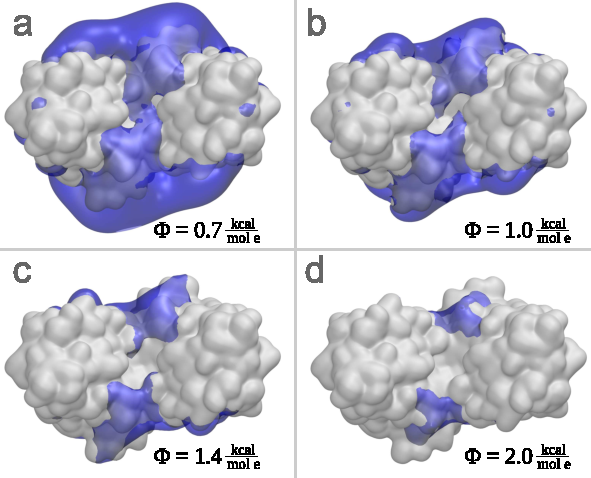
\includegraphics[width=1.0\textwidth]{gfx/bspred/il10_top_coulomb_isosurfaces_different_values_03_ds.pdf}
\caption[]{
Isosurface representation of IL-10's Coulomb potential (blue), shown for
multiple isovalues $\Phi$. The molecular surface of the IL-10 dimer is
shown in gray (structure taken from PDB ID 2ILK).
}
\label{fig:bspred:il10_multi_iso}
\end{figure}

The procedure of changing electrostatic isosurface with increasing isovalue is
depicted in \cref{fig:bspred:il10_multi_iso}. The characteristic isovalue has
been narrowed down to \SI{2.0}{\kilo\calory\per\mole\per\elementarycharge},
which is weaker than even the lowest isovalue shown for FGF2 in
\cref{fig:bspred:fgf2_multi_iso}. Hence, IL-10's Coulomb attraction for GAGs
is qualitatively different from FGF2's and SDF-1's --- it is much weaker.
Comparison of the isosurfaces in figures \ref{fig:bspred:fgf2_multi_iso}a and
\ref{fig:bspred:il10_multi_iso}d (different protein, comparable isovalue) shows
how different IL-10 and FGF2 are with respect to their capability of attracting
GAGs through larger distances. Notably, IL-10's characteristic isovalue of
\SI{2.0}{\kilo\calory\per\mole\per\elementarycharge} still represents a
\textit{significant} attraction for GAGs being in contact with IL-10, with the
energy per test charge being about three times larger than the thermal energy at
room temperature.

While the strength of IL-10's Coulomb potential can be described in simple
terms, its topology displays rather special features. In
\cref{fig:bspred:il10_multi_iso}a a well-ordered isosurface can be observed,
i.e.\ an isosurface with homogeneous appearance and no scattering. Generally,
the volume surrounding IL-10 can be subdivided in two parts: one part being
affected by electrostatic attraction for GAGs (the blue part), and a rather
unaffected part (where the molecular surface is not covered by the Coulomb
potential isosurface at all), indicating a certain electrostatic polarity on
IL-10's global scale. The electrostatic potential isosurfaces are symmetrically
assembled, according to the two-fold rotational symmetry of the IL-10 dimer.
GAGs are directional molecules (extended in one dimension). The isosurfaces
shown in panels a and b of \cref{fig:bspred:il10_multi_iso} suggest that IL-10's
Coulomb potential tends to align a GAG's direction of longest extent either
along its \enquote{side-side} direction, or along the groove of the V-shape,
which is in \enquote{front-back} direction (following the V-shape nomenclature
as introduced in \cref{background:structureil10system}, and the perspective
shown in \cref{fig:bspred:il10_multi_iso} is from the top of the V towards its
bottom). With increasing isovalue the origin of this attraction can be narrowed
down: \cref{fig:bspred:il10_multi_iso}d shows two \textit{distinct} surface
patches of considerable electrostatic attraction.

In \cref{bspred:general_conclusions} I concluded that whenever a distinct region
of significant electrostatic attraction is observable, then this is the place
where a GAG most likely binds. In case of IL-10, one distinct region was just
identified (occurring twice as of IL-10's spatial symmetry). The distribution of
IL-10's Coulomb potential in space therefore provides strong evidence that if
GAGs interact with IL-10, the interaction is most likely centered on the two
blue spots shown in \cref{fig:bspred:il10_multi_iso}d. While the strength of
this attraction has been identified as weaker than in case of the exemplary
protein-GAG systems discussed before, it is still significantly larger than the
thermal energy at \SI{300}{\kelvin}.


\begin{figure}
\centering
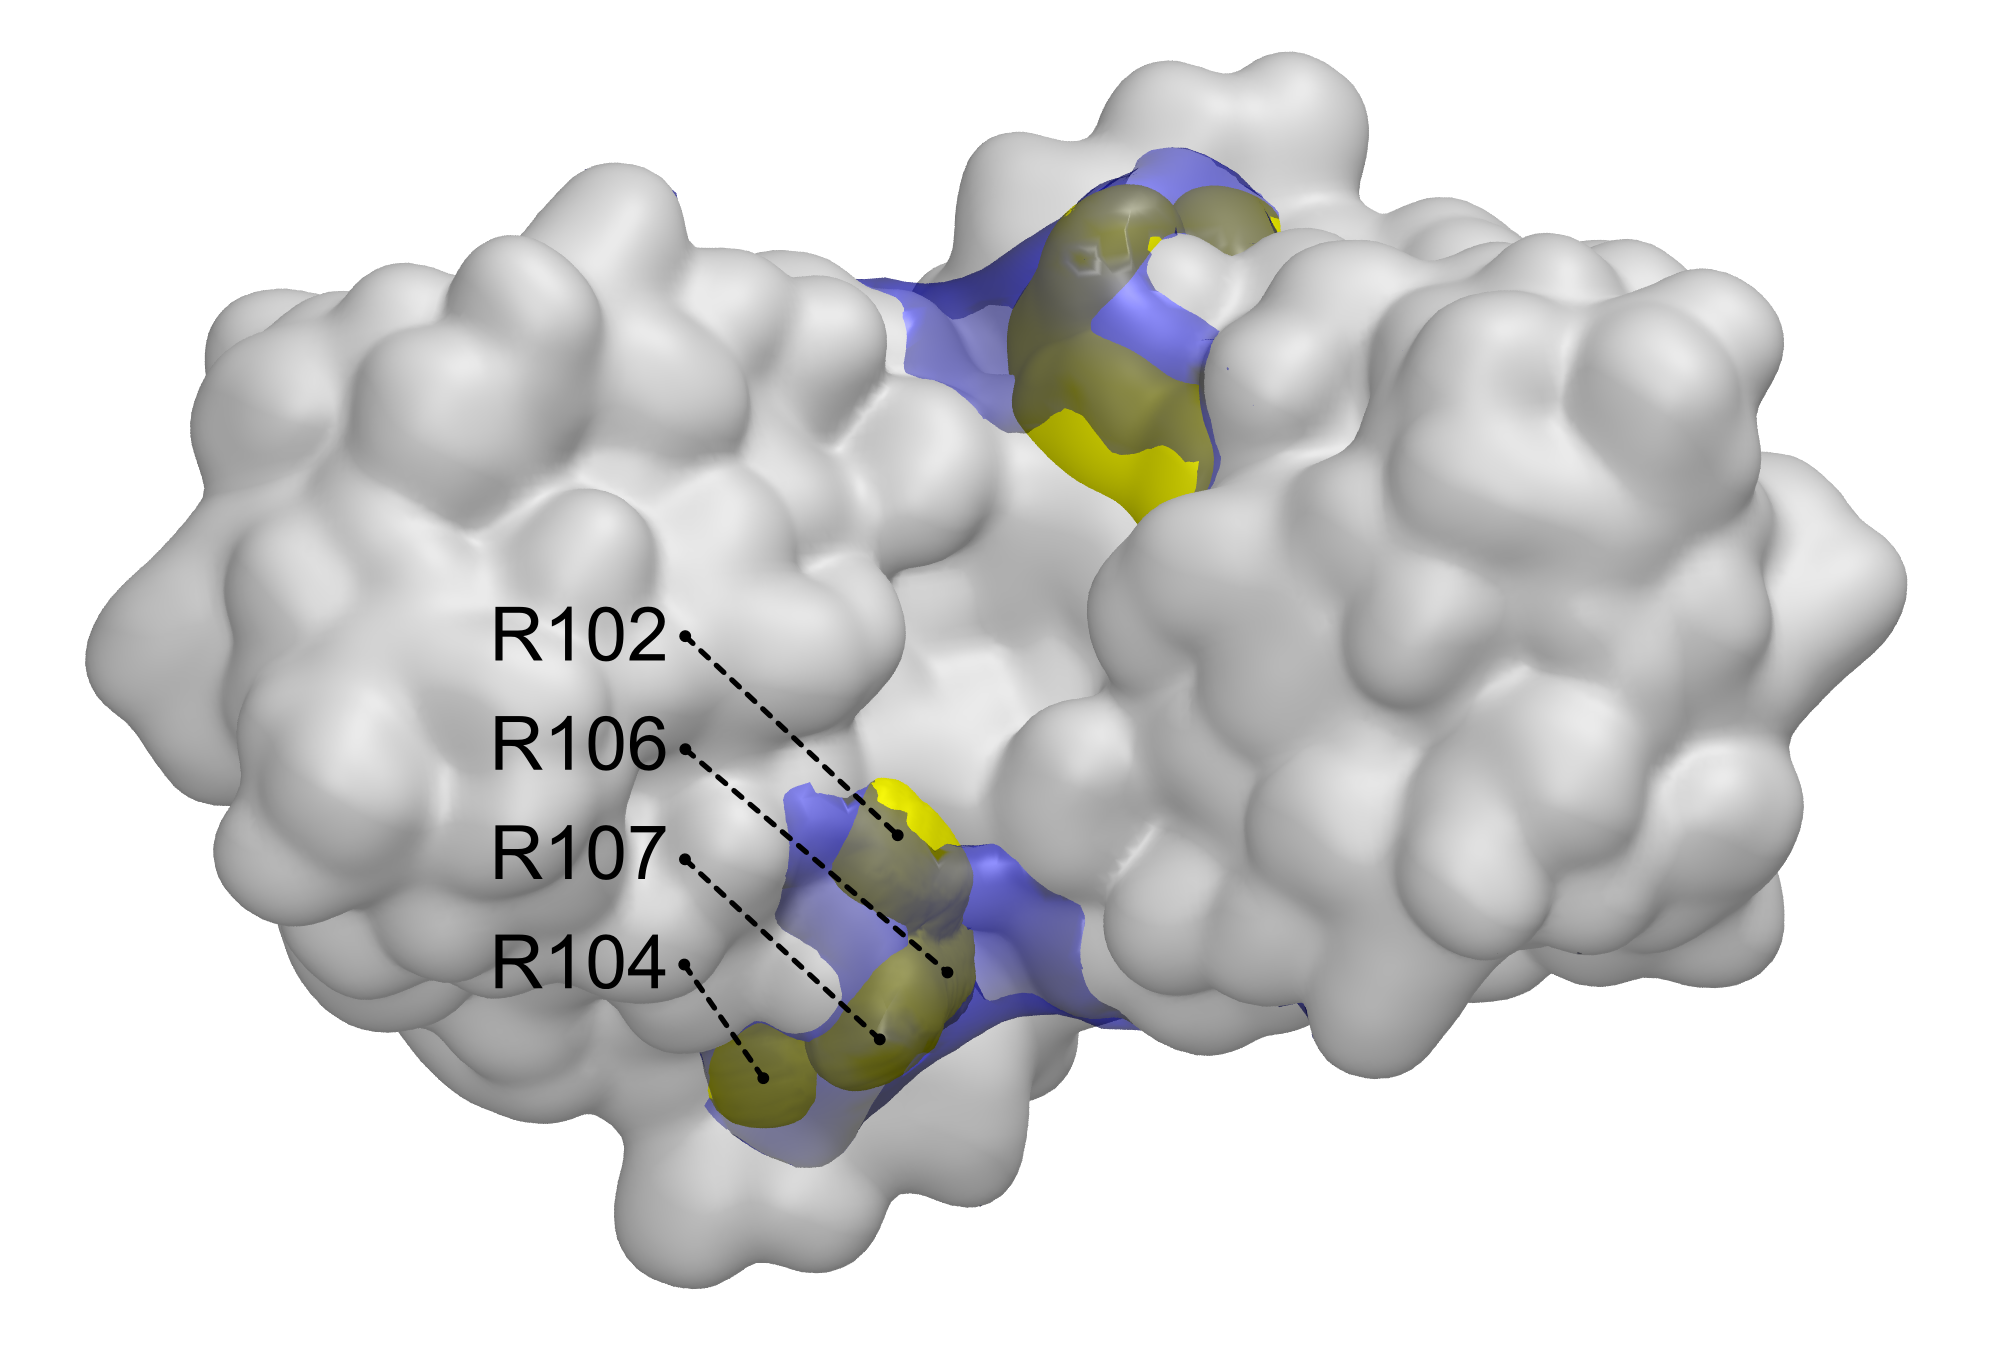
\includegraphics[width=0.9\textwidth]{gfx/bspred/SI_figure_IL-10_coulomb_isosurface_1_9kcalmol.png}
\caption[]{
Isosurface representation of IL-10's Coulomb potential with the isovalue $\Phi =
\SI{1.9}{\kilo\calory\per\mole\per\elementarycharge}$ (blue). The molecular
surface of the IL-10 dimer is shown in gray, the molecular surface of arginines
102, 104, 106, 107 is shown in yellow (structure taken from PDB ID 2ILK). This
representation allows to see where the Coulomb potential (for a given isovalue)
protrudes into space further than the molecular surface, and has been shown to
provide useful evidence about where GAGs bind to a protein (see
\cref{bspred:general_conclusions}. Hence, IL-10-GAG interaction most likely
takes place within the two symmetrically arranged regions indicated here.}
\label{fig:bspred:il10_estatic_pred}
\end{figure}

The GAG-attractive Coulomb potential of the putative binding region mainly
arises from four arginine residues in the sequence of the human IL-10 monomer:
R102, R104, R106, R107, labeled in \cref{fig:bspred:il10_estatic_pred}. A closer
look at this region reveals that R107 is particularly solvent-exposed, i.e.\ it
could serve as key residue in IL-10-GAG interaction. It is quite interesting to
note that already in one of the first structural descriptions of IL-10 back in
1995 \cite{Zdanov1995}, Zdanov et al.\ characterized this region as being
special:

\begin{adjustwidth}{1.5cm}{1.5cm}
\textit{%
\enquote{The C-terminal part of helix D has a patch of positively
charged residues (K99, R102, R104, R106, R107, H109 and R110). These seven
residues are mostly conserved in IL-10 between species and form a positively
charged surface [\dots]. This patch appears to be a specific feature of IL-10.}}
\end{adjustwidth}


Overall, I am quite certain that the discussed region plays a major role in
IL-10-GAG interaction. However, a GAG-IL-10 binding region prediction is not
reported for the first time. In \cite{mulloy_forster_2008_4helixcytokines},
where AutoDock 2.4 \cite{autodock24} was applied in a virtual screening fashion
to a large set of cytokines, the authors list the IL-10 residues R102, R106,
R107, N116, K117, K119, and K125 as being important for GAG binding, but at the
same time state that a \enquote{detailed analysis of the predicted binding sites
has been avoided as being premature in the absence of experimental data}. The
latter is in line with a central aspect of this chapter --- a prediction is only
useful when one is able to rationally derive its applicability and to assess its
significance. Otherwise, both validation or invalidation of the prediction with
the help of an experiment \textit{would not improve theoretical knowledge}:
proving the prediction right must be considered coincidence, proving the
prediction wrong would not provide fundamental insights about why the applied
model was insufficient to describe the system. Again, alone the electrostatic
properties of IL-10 nicely explain the docking results obtained in
\cite{mulloy_forster_2008_4helixcytokines}.

In \cite{salek_ardakani_2000}, where IL-10 was shown to bind heparin, the
authors note that IL-10 residues 105 to 110 (LRRCHR) match the pattern XBBXBX,
which was earlier published as one of various protein-GAG binding site
\enquote{consensus sequences} (where B represents a cationic amino acid residue
and X represents an uncharged one). The idea that protein-GAG interaction should
be governed by such consensus sequences has been proposed and pushed forward by
various authors in the 1990s \cite{mccaffrey_1992,
cardin_weintraub_1989,fromm_1997,caldwell_1996,hileman_1998}. If that was the
case, scanning proteins for such sequence fragments would be a powerful
protein-GAG binding region prediction method. However, in fact, the interaction
between two molecules is clearly governed by the assembly of atoms in space,
i.e.\ by their \textit{structure} rather than their \textit{sequence}. In
consequence, protein sequence information is not suitable for making resilient
protein-GAG binding region predictions. This view is supported by Forster and
Mulloy who state that \enquote{though some 'consensus sequences' for heparin
binding have been identified, they are neither necessary nor sufficient to
define a heparin binding site} \cite{hp_binding_sites_mulloy_2006}. The Coulomb
potential analysis method presented here, on the other hand, used protein
\textit{structure} information as its basis.

In case of IL-10, the consensus sequence approach and the prediction made here
seem to roughly match. The reason is that the named \enquote{consensus sequence}
is a local agglomeration of positively charged amino acid residues in IL-10: it
is purely the local density of positively charged residues that is responsible
for the compliance of both predictions. Hence, the order of residues in the
\enquote{consensus sequence} is not important for the two predictions to match,
diminishing one main aspect of the \enquote{consensus sequence} idea. The fact
that both predictions match can be considered a matter of coincidence.

% reducing the idea of a certain required residue pattern reflected by the
% to absurdity.

% a special arrangement of the side chains could
%abolish the strong electrostatic attraction for negatively charged molecules. In
%that case, the sequence fragment would still match a so-called consensus
%sequence, whereas Coulomb potential evaluation would

\subsection{Conclusions}
The strength of IL-10's Coulomb attraction for GAGs has been identified to be
significantly weaker than in case of exemplary protein-GAG systems such as
FGF2-HP. Nevertheless, with its magnitude being about three times larger than
the thermal energy at room temperature it can be considered as still being
significant. The origin of this attraction has been revealed to be a distinct
region centered on R102, R104, R106, R107 of the human IL-10 monomer --- a
region that had previously been characterized as a specific feature of IL-10
\cite{Zdanov1995}. All in all, the discussed region can be assumed to play a
major role in IL-10-GAG interaction.